\section{Formal proof structures}
\label{sc:formal}

Present here the auxiliary state annotations. The colors. The automata
describing how colors evolve. Probably in the following order:

\begin{enumerate}
\item Start by presenting histories and timestamps. Discuss self/other
  histories, and joint histories. Say that timestamps identify events,
  i.e. linearization points of an event. While timestamps are natural
  numbers, and the nat ordering is the \emph{real-time} ordering of
  the events, this is not the logical ordering we want. Thus, in the
  joint state we will keep the list of timestamps representing the
  logical order of events, but use the timestamps as a kind of
  temporal pointer that identifies the events. We keep this info in
  the joint state, because we want this order to be modifiable by all
  threads that call a scanner.

\item The above components (i.e., histories, timestamps and logical
  order) are sufficient to describe the spec for write and scan.  Do
  so, and describe them. Emphasize the following points here.

 %% \is{Do we have an agreement on what these specs are?}\an{We have a
 %%   working set of specs, which looks good to me. I'll type them up
 %%   below.}
 
  \begin{itemize}
  \item Unlike in linearizability, we don't record in histories the
  operations, such as scan, which don't modify the state. It suffices
  merely to say \emph{in the spec of scan}, that after the scan is
  done, the returned timestamp fixes the order of all the events prior
  to the scan.

  \item The spec for write says that all the events prior to write
  will never be reordered after write. I guess we can call this
  ``sequential consistency''?

\item We use small \emph{temporal} footprint specification, in that we
  assume that the input history of both write and scan are empty. This
  is not a loss of generality, because the same kind of framing from
  separation logic applies here as well.  \is{I think it's okay to
    give a large footprint spec right away without going into the
    framing discussion. We will need it like that later for clients
    anyway.}
  \end{itemize}

\item We need additional information in the auxiliary state, in order
  to be able to prove the above specs.

  We need to keep track of end-points of the write operations. This is
  necessary in order to be able to prove that the write will never be
  reordered with the events that terminated, in the same thread,
  before the write started. This is essentially a stability
  property. Another way to achieve it is by tracking thread ids, but
  we find it interesting that keeping end-times is more general, and
  allows us to dispense with thread ids. Consequently, we will be able
  to very easily reason about clients which arbitrarily nest parallel
  compostion.  \an{I personally find this very interesting. While in
    linearizability, keeping track of the two endpoints of the program
    is the default mode of operation, in our setting, this is just a
    proof technique to stabilize the sequential ordering. I wonder if
    the inventors of linearizability have introduced the property for
    exactly the same reason. If so, they shouldn't have needed thread
    id's, I think.}

\item We need colors, in order to identify the various stages of
  interaction between writer and scanner. Describe them here. Describe
  the invariants that relate them. \gad{We need colors to define the
    Stable-- or fixed -- logical ordering so the order of this items
    might change when this is written. So this should go above, I
    guess.}

  \gad{TO DO: Describe projections, G+.Y?.R* and red shift color
    invariants}.
  
\item We need to describe how re-link works, and how it preserves the
  invariants.  \gad{We have nice drawings from the talk and my notes
    that we could re-use if we have both the time and
    space}. \gad{Will do that, and a proof sketch}
  
%% \item Give some proof outlines? \is{No. It's PODC. Check the Hindsight
%%   paper for the inspiration.}

%% \item Do we need a background section on FCSL in order to explain
%%   the proof outline? \is{Hell, no.} Maybe not, since neither
%%   writer, nor the scanner, contain parallel composition, framing,
%%   or hiding.

 %% \gad{Well I guess this depends on how deep we go explaining the
 %%   colors. If we present the automatons we need to give some intuition
 %%   on what the tranistions are. We could do this informally here, and
 %%   then have an appendix with the ``FCSL primer'' from previous paper,
 %%   plus some details about this concurroid in particular.}

\end{enumerate}

\newcommand{\selfsub}{\mathsf{S}}
\newcommand{\othersub}{\mathsf{O}}
\newcommand{\jointsub}{J}
\newcommand{\histS}{\hist_\selfsub}
\newcommand{\histO}{\hist_\othersub}
\newcommand{\histJ}{\hist_\jointsub}
\newcommand{\jleq}{\mathop{\leq_\jointsub}}
\newcommand{\jle}{\mathop{<_\jointsub}}
\newcommand{\jge}{\mathop{>_\jointsub}}
\newcommand{\hempty}{\mathsf{empty}}


\makeatletter
\DeclareRobustCommand{\cev}[1]{%
  \mathpalette\do@cev{#1}%
}
\newcommand{\do@cev}[2]{%
  \fix@cev{#1}{+}%
  \reflectbox{$\m@th#1\vec{\reflectbox{$\fix@cev{#1}{-}\m@th#1#2\fix@cev{#1}{+}$}}$}%
  \fix@cev{#1}{-}%
}
\newcommand{\fix@cev}[2]{%
  \ifx#1\displaystyle
    \mkern#23mu
  \else
    \ifx#1\textstyle
      \mkern#23mu
    \else
      \ifx#1\scriptstyle
        \mkern#22mu
      \else
        \mkern#22mu
      \fi
    \fi
  \fi
}


\paragraph{Specs for snapshot methods.}

This is the spec we are currently going with. Germ\'an is now checking
if this all works, but we've arrived to this after quite a lot of
failures, and this setup should be able to overcome all of
them. Hopefully, no new ones arise. But some small adjustments may be
needed.

\[
\begin{array}{l}
\mathtt{write}\ (p : \mathtt{ptr}, n : \mathtt{int}) : 
\!\!\!\begin{array}[t]{l}
\{\hists = \hempty \wedge h \subseteq \histO \wedge \omega \subseteq \jleq\}\\
\{\exists t\ldot\, \hists = t \mapsto (p, n) \wedge h \subseteq \histO \wedge
  \omega \subseteq \jleq\,{\wedge}\, \mathsf{dom}\ h \subseteq \cev{t}
        \setminus \{t\}\}
\end{array}\\
%
\mathtt{scan} : 
\!\!\!\begin{array}[t]{l}
\{
\hists = \hempty \wedge h \subseteq \histO \wedge \omega \subseteq \jleq\}\\
\{\hists = \hempty \wedge h \subseteq \histO \wedge \omega \subseteq
        \jleq \wedge \hbox{}\\
\hphantom{\}}
  \exists t\ldot\, \mathsf{dom}\ h \subseteq \cev{t} \wedge
  \mathsf{total}\ {\cev{t}} \wedge 
 \cev{t} \hunion \vec{t} = \mathsf{dom}\ (\histO
        \hunion \histJ)
        \wedge r = \mathsf{eval}\
        {\cev{t}}
\}
\end{array}
\end{array}
\]

Here, I used the following abbreviations:

\[
\begin{array}{lcl}
\cev{t} & =  & \{t' \in \mathsf{dom} (\histO \hunion \histJ)
\mid t' \jleq t\}\\
\vec{t} & = & \{t' \in \mathsf{dom} (\histO \hunion \histJ) 
\mid t' \jge t\}
\end{array}
\]
\gad{Adjusments are coming in}
Let me explain.

We arrange the actions and the concurroid so that the history entries
$\histS$ and $\histO$ keep the timestamps for the writes that
\emph{have finished}, i.e., their endpoints appear before the
currently largest timestamp. There's also the history $\histJ$, which
keeps the writes that haven't yet terminated. Upon termination, these
writes are moved to $\histS$, by their owner thread.

The order $\jleq$ is a \emph{partial} order on timestamps. In the
joint state, we keep a total order of timestamps, each one identifying
a separate write. This includes the writes that finished (i.e., are in
$\histS \hunion \histO$), or are still ongoing (i.e., are in
$\histJ$). Some timestamps in that total order are subject to
rearrangement. Hence, the total order itself is not stable,
as-is. Here, $\jleq$ is the partial suborder of that order,
\emph{which is stable}. Inside the proof, $\jleq$ is defined to order
all the green timestamps, as well as timestamps that corresond to
non-overlapping writes. (Non-ovelappnes can be determined, because we
now also keep the ending timestamp for each event, but we do so in a
separate piece of joint state, which is not exposed to the clients).


Then, the spec for {\tt write} says: (1) the history of others only
grows, (2) the stable part of the order grows as we progress
($\omega \subseteq \jleq$), and (3) the time-stamp $t$ at which the
write happens, appears \emph{strictly after} all the writes in $h$
($\mathsf{dom}\ h \subseteq \cev{t} \setminus\{t\}$).

Notice that $\cev{t}$ takes the timestamps of all events (finished or
not), that are smaller (or equal) to $t$, while $\vec{t}$ takes the
remaining ones.

Thus, the spec is quite subtle. Notice: it allows for some of the
events in $h$ to be reordered themselves, \emph{after} {\tt write}
finishes (i.e., $h$ doesn't have to be all included into the domain of
$\jleq$). Indeed, some of these events from $h$ may be collored yellow
or red, so we don't know their final order at the time {\tt write}
finishes. However, we know that, even if they are reordered in the
future, they won't be reorder to appear \emph{before} $t$. This will
be ensured by the invariant of the concurroid that non-overlapping
events are not reordered, and the fact that the events from $h$ indeed
do not overlap with $t$, as they have all terminated before $t$ starts
(by definition, since they appear in $\histS \hunion \histO$).


The spec for {\tt scan} says: (1) again, the history of others and the
stable part of the order only grows, (2) the timestamp $t$ at which we
logically pretend to have performed the scan appears later (or at the
last moment) of the events that already happend
($\mathsf{dom}\ h \subseteq \cev{t}$), (3) the set $\cev{t}$ is
totally ordered by $\jleq$; that is, any two elements of the set are
ordered by $\jleq$. Hence, $\cev{t}$ represent the \emph{chain} of
events leading to the scan. Notice, because $\jleq$ is stable, this
means that \emph{there will be no reorderings in this chain
  anymore}. Indeed, an aposteriori reordering of the chain may
invalidate the results of the scan, so we have to prohibit it. (4) $t$
is related to all the timestamps. That is, if we take $\cev{t}$ and
$\vec{t}$ together, that exhausts all the timestamps. This ensures
that no future timestamp will be reordered \emph{before $t$} (i.e.,
spliced into the chain $\cev{t}$), as that too would invalidate the
already obtained scan. Elements of $\vec{t}$ need not form a chain, as
some events may yet to be ordered wrt.~each other, though they all
appear after $t$. (5) Finally, evaluating the writes that are elements
of $\cev{t}$ gives us the result $r$ that {\tt scan} returns.

% A stub for the re-linking figure.
\begin{figure}
\begin{subfigure}[t]{0.48\textwidth}
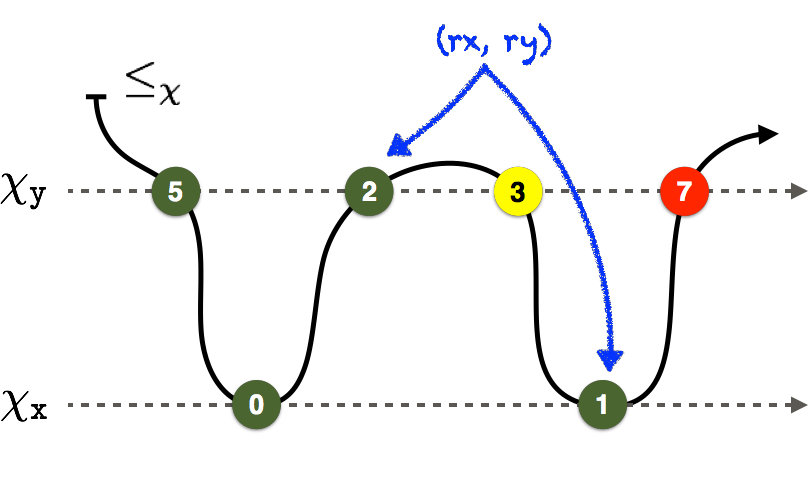
\includegraphics[height=5cm]{res/before-relink-trans}
\caption{\label{fig:relink:before} Before re-link}
\end{subfigure} \hfill
\begin{subfigure}[t]{0.48\textwidth}
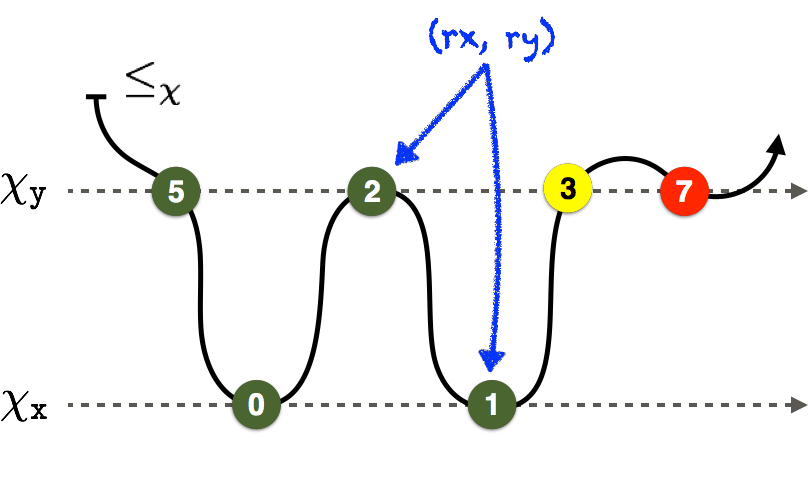
\includegraphics[height=4.5cm]{res/after-relink-trans}
\caption{\label{fig:relink:after} After re-link}
\end{subfigure}%
%
\caption{\label{fig:relink} Atomic re-link: $(rx,ry)$ points to the
  snapshot that will be returned by {\tt scan}}
\end{figure}

\gad{FIX ME: subfigure (b) is incorrectly drawn! 1 and 3 are swapped
  in Real Time as well!!!}

%Fix me: The yellow should be painted red after relink, if we decide
%to go for the (green - red) split for t\left t\right after re-link.
%Though, this would not be stable after we release the lock for scan,
%so why bother. Painting the t|left chain green will suffice, as it
%will be stable.

% Fix me: red marbles have different font colors :(


\paragraph{Re-link}
We might want to explain here how re-link works through
Figure~\ref{fig:relink}, and revisit the example from the previous
section given the colors and the invariants. \gad{The figure might
  change to include the redzone invariant as well, as the endpoints if
  we need to}

% Bear in mind that this picture will feature the internal, complete
% order \leq_{\chi} -- the hourglass in the slides-- which corresponds
% to the full ordering in the joint state. I mean, I'd probably have
% to present it anyway, as it is part of \leq_{J}.


